\section{Bottom-up syntax analysis}

To systematically create a bottom-up syntax analyzer, the following steps are used:
\begin{enumerate}
    \item Construction of the pilot graph that directs the bottom-up syntax analyzer.
        Each macro-state within the pilot encompasses all relevant information about potential phrase forms reaching that state with look-ahead.
        Each macro-state (m-state) incorporates machine states with look-ahead, indicating the expected characters during reduction.
    \item Thread generation from m-states: utilize the m-states to generate analysis threads in the stack, representing potential derivations.
        These threads correspond to machine network computations or paths with $\varepsilon$-arcs at each machine change, labeled with the scanned string.
    \item Verification of determinism conditions: check for determinism conditions on the pilot graph, including shift-reduce conflicts, reduce-reduce conflicts, and convergence conflicts.
    \item Determinism test: if the determinism test is successfully passed, the bottom-up syntax analyzer can analyze the string deterministically.
    \item Utilization of pilot graph and stack information: the bottom-up syntax analyzer utilizes the information stored in both the pilot graph and the stack for analysis.
\end{enumerate}

\begin{definition}[\textit{Set of initials}]
    The set of initials represents characters starting from state $q_A$ of machine $M_A$ in the network $M$: 
    \[\textnormal{Ini}(q_A)=\textnormal{Ini}(L(q_A))=\{a \in \Sigma|a\Sigma^{*}\cap L(q_A) \neq \varnothing\}\]
\end{definition}
This set is defined based on three possible cases:
\begin{itemize}
    \item $a \in \textnormal{Ini}(q_A)$ if exists an arc $q_A \overset{a}{\rightarrow}r_A$. 
    \item $a \in \textnormal{Ini}(q_A)$ if exists an arc $q_A \overset{B}{\rightarrow}r_A$ and $a \in \textnormal{Ini}(0_B)$. 
    \item $a \in \textnormal{Ini}(q_A)$ if exists an arc $q_A \overset{B}{\rightarrow}r_A$ and $L(0_B)$ is nullable, and $a \in \textnormal{Ini}(r_A)$.
\end{itemize}
\begin{example}
    Consider the given grammar:
    \[\begin{cases}
        S \rightarrow Aa \\
        A \rightarrow BC \\
        B \rightarrow b|\varepsilon \\
        C \rightarrow c|\varepsilon
    \end{cases}\]
    The corresponding machine net is illustrated below:
    \begin{figure}[H]
        \centering
        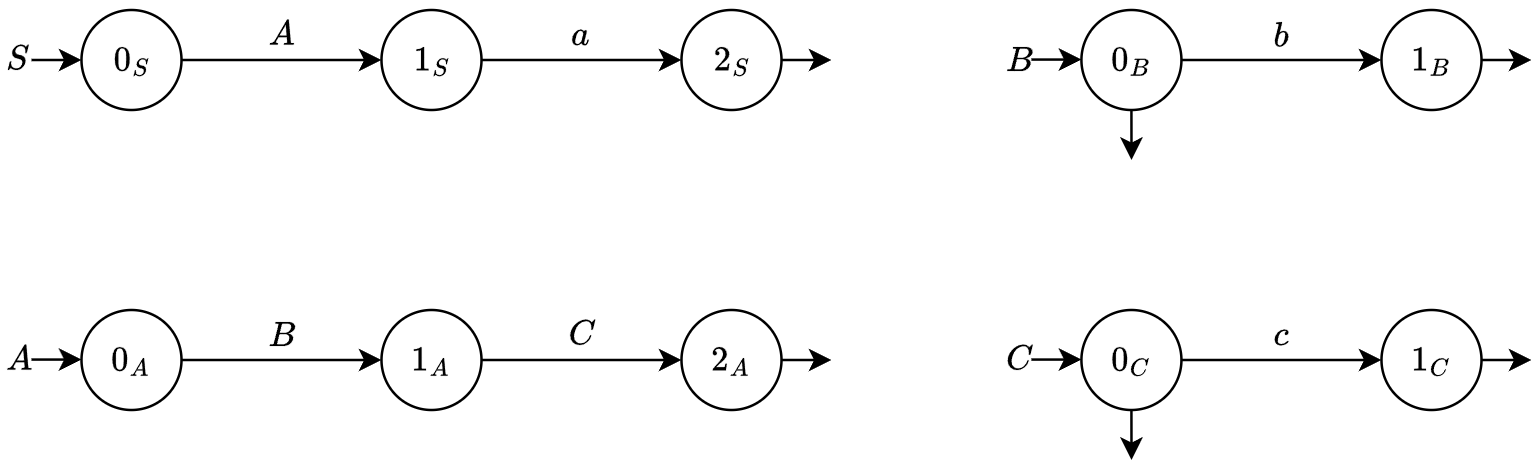
\includegraphics[width=0.75\linewidth]{images/net1.png}
    \end{figure}
    To determine the set of initials for state $S_0$, the following states are examined:
    \begin{itemize}
        \item $\textnormal{Ini}(0_S)=\textnormal{Ini}(0_A) \cup \textnormal{Ini}(1_S)$ because $L(0_A)$ is nullable. 
        \item $\textnormal{Ini}(0_A)=\textnormal{Ini}(0_B) \cup \textnormal{Ini}(1_A)$ because $L(0_B)$ is nullable. 
        \item $\textnormal{Ini}(1_A)=\textnormal{Ini}(0_C) \cup \textnormal{Ini}(2_A)$ because $L(0_C)$ is nullable. 
    \end{itemize}
    The final result is: 
    \[\textnormal{Ini}(0_S)=\{b\} \cup \{c\} \cup \{a\}\]
\end{example}
\begin{definition}[\textit{Item}]
    An item is represented as $\left\langle q_B,a\right\rangle$ in $Q \times (\Sigma \cup \{\dashv\})$.
\end{definition}
Two or more items sharing the same state can be consolidated into a single item. 
An item associated with a machine's final state is termed a reduction item.
\begin{definition}[\textit{Closure}]
    The closure function computes a form of closure for a set $C$ of items with look-ahead.
\end{definition}
To find the closure of $C$, the following recursive clause is applied iteratively until a fixed point is reached (initially set as closure $\textnormal{closure}(C)=C$): 
\[\left\langle 0_B,b\right\rangle \in \textnormal{closure}(C) \textnormal{ if }
\begin{cases}
    \exists \textnormal{ candidate } \left\langle q,a\right\rangle \in C \textnormal{ and} \\
    \exists \textnormal{ arc } q \overset{B}{\rightarrow} r \textnormal{ in } \mathcal{M} \textnormal{ and} \\
    b \in \textnormal{Ini}(L(r)a)
\end{cases}\]
\begin{definition}[\textit{Shift operation}]
    The shift operation is defined as: 
    \[\begin{cases}
        \theta(\left\langle p_A,\rho\right\rangle,X)=\left\langle q_A,\rho\right\rangle \textnormal{ if the arc } p_a \overset{X}{\rightarrow} q_a \textnormal{ exists} \\
        \textnormal{the empty set otherwise}
    \end{cases}\]
\end{definition}
A shift corresponds to a transition in a machine $Y$: 
\begin{itemize}
    \item If $X=c$ is a terminal symbol, then the shift is a bottom-up syntax analyzer move that reads a character $c$ from the input.
    \item If $X$ is a non-terminal symbol, then the shift is a bottom-up syntax analyzer $\varepsilon$-move after a reduction $z \rightarrow X$, and it does not read any input.
    \item Machine $Y$ undergoes a transition with a nonterminal label $X$. 
    \item The analysis continues after recognizing an input substring $z \in L (X)$ derivable from the nonterminal $X$. 
\end{itemize}
The shift operation extends to sets of items (denoted as m-state): 
\[\vartheta(C,X)=\bigcup_{\forall \gamma \in C} \vartheta(\gamma,x)\]

\subsection{Pilot graph}
\paragraph*{Pilot graph}
The pilot graph is a deterministic finite state automaton denoted as $\mathcal{P}$. 
It is characterized by the following components:
\begin{itemize}
    \item The set $R$ of m-states. 
    \item The pilot alphabet, which is the union $\Sigma\cup V$ of terminal and non-terminal alphabets, also referred to as grammar symbols.
    \item The initial m-state, $I_0$, defined as the closure of $\left\langle 0_S, \dashv \right\rangle$.
    \item The m-state set $R={I_0,I_1,\dots}$ and the state-transition function $\theta:R \times (\Sigma \cup V) \rightarrow R$, computed starting from $I_0$. 
\end{itemize}
The construction of the pilot graph is incremental and concludes when no further changes occur.
It lacks final states as it does not recognize strings.
The items in each m-state $I$ of the pilot are divided into two groups:
\begin{itemize}
    \item \textit{Base}: contains items obtained after a shift, representing non-initial states.
    \item \textit{Closure}: contains items obtained after a closure, representing initial states.
\end{itemize}
\begin{definition}[\textit{M-state kernel}]
    The m-state kernel of an m-state $I$ is defined as the set of m-states of $I$ without look-ahead.
\end{definition}
\begin{algorithm}[H]
    \caption{Pilot graph construction algorithm}
        \begin{algorithmic}[1]
            \State $R^{'} \leftarrow \{I_0\}$
            \While {$R \neq R^{'}$}
                \State $R \leftarrow R^{'}$
                \For {each m-state $I \in R$ and symbol $X \in \Sigma \cup V$}
                    \State $I^{'} \leftarrow \textnormal{closure}(\vartheta(I,X))$
                    \If {$I^{'} \neq \varnothing$}
                        \State add arc $I \overset{X}{\rightarrow} I^{'}$ to the graph of $\vartheta$
                        \If {$I^{'} \notin R$}
                            \State add m-state $I^{'}$ to the set $R^{'}$
                        \EndIf
                    \EndIf
                \EndFor
            \EndWhile
        \end{algorithmic}
\end{algorithm}
\begin{example}
    Consider the grammar: 
    \[\begin{cases}
        E \rightarrow T^{*} \\
        T \rightarrow '('E')'|a
    \end{cases}\]
    The corresponding machine net is illustrated below:
    \begin{figure}[H]
        \centering
        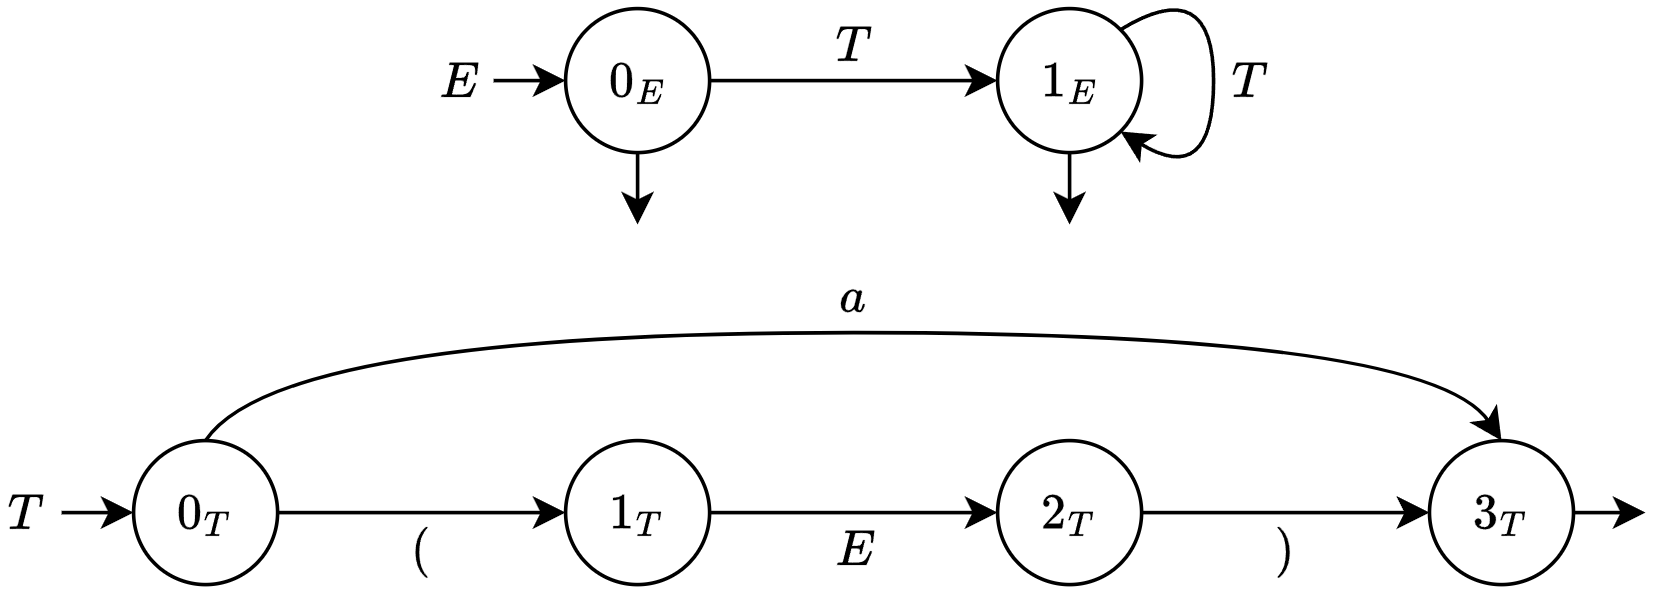
\includegraphics[width=0.5\linewidth]{images/net2.png}
    \end{figure}
    Applying the previous algorithm yields the following pilot graph:
    \begin{figure}[H]
        \centering
        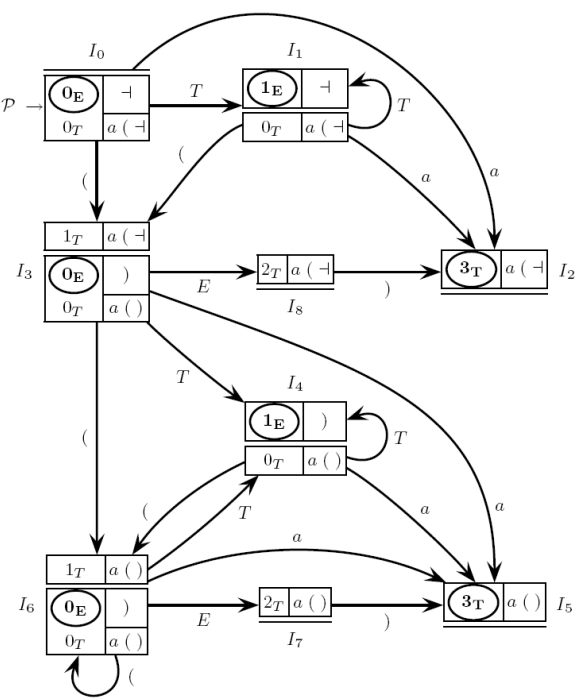
\includegraphics[width=0.4\linewidth]{images/pil.png}
    \end{figure}
    It is noteworthy that the kernel-equivalent m-states are:
    \[(I_3, I_6),(I_1, I_4),(I_2, I_5),(I_7, I_8)\]
\end{example}
If an m-state includes an item with a final state, the bottom-up syntax analyzer executes a reduction move.
The look-ahead of the reduction item specifies the input characters anticipated at the time of reduction.
The bottom-up syntax analyzer examines the current input character $cc$ and takes the following actions:
\begin{itemize}
    \item If $cc \in \textnormal{look-ahead}$, the bottom-up syntax analyzer performs a reduction.
    \item If $cc$ is not in the look-ahead set, the bottom-up syntax analyzer reads input character $cc$ and shifts along an arc labeled with $cc$.
    \item In any other case, the bottom-up syntax analyzer halts and rejects.
\end{itemize}

\subsection{ELR(1) method}
The conditions for applying the ELR(1) method are the absence of:
\begin{itemize}
    \item \textit{Shift-reduce conflicts}: when there is a reduction item with look-ahead that intersects with the terminal symbols on the outgoing arcs. 
        In the presence of such conflicts, the bottom-up syntax analyzer faces ambiguity in choosing between shifting and reducing.
    \item \textit{Reduce-reduce conflicts}: when two or more reduction items with look-ahead overlap. 
        In cases of these conflicts, the bottom-up syntax analyzer encounters difficulty in selecting the appropriate reduction.
    \item \textit{Convergence conflicts}: When an m-state contains two or more items with two or more next states defined for a symbol $X$ (terminal or not). 
        In the presence of these conflicts, the bottom-up syntax analyzer struggles to resolve the reduction choice among the converging paths.
\end{itemize}
\begin{definition}[\textit{Transitions convergence}]
    A multiple transition is considered \emph{convergent} if: 
    \[\delta(p,X)=\delta(r,X)\]
\end{definition} 
\begin{definition}[\textit{Trnasitions conflict}]
    A convergent transition is labeled as having a \emph{conflict} if: 
    \[\pi \cap \rho \neq \varnothing\]
\end{definition}

\subsection{Bottom-up syntax analyzer's workflow}
The workflow of the bottom-up syntax analyzer unfolds as follows:
\begin{enumerate}
    \item The bottom-up syntax analyzer scans a string and executes a series of shift and reduction moves.
    \item Groups of items are pushed onto the stack, commencing with those in the initial pilot m-state.
    \item Each m-state item transforms into a 3-tuple by incorporating a backward-directed pointer. 
        This pointer aids in reconstructing the various analysis threads constructed in parallel.
    \item The decision to scan or reduce is made by the bottom-up syntax analyzer based on the look-ahead in the pilot.
    \item If the ELR(1) condition is satisfied, the bottom-up syntax analyzer operates deterministically.
\end{enumerate}
It's crucial to note that the length of the reduction handle is not fixed, allowing a rule to generate phrases of unbounded length. 
The reduction handle length is determined dynamically at reduction time using the pointers. 
The pointer chain is traced backward to the point where the analysis thread originated. 
A pointer value $\perp$ identifies a thread start point, and all closure items have a pointer value $\perp$, designating them as the start points of new threads.
A three-tuple with a pointer different from $\perp$signifies the continuation of an already initiated thread, and these non $\perp$ pointers are represented as $\#i$, where $\#i$ indicates the pointer is targeted to the $i$-th item (from top to bottom) in the previous stack element.

\subsection{Computational complexity}
When examining a string $x$ with a length of $n = \left\lvert x \right\rvert $, the stack's size is at least $(n + 1)$. 
To determine the count of bottom-up syntax analyzer moves, we consider the following factors:
\begin{itemize}
    \item The number of terminal shifts, denoted as $n_T$.
    \item The number of nonterminal shifts, denoted as $n_N$.
    \item The number of reductions, denoted as $n_R$.
\end{itemize}
These variables are interconnected in the following manner: the count of terminal shifts corresponds to the string's length, and the number of nonterminal shifts equals the number of reductions. 
Consequently, the total number of bottom-up syntax analyzer moves can be expressed as:
\[n_T+n_N+n_R=n+2n_R\]
Moreover:
\begin{itemize}
    \item The count of reductions involving one or more terminals ($A \rightarrow a$) is less or equal to $n$. 
    \item The count of reductions of null type ($A \rightarrow \varepsilon$) and copy type ($A \rightarrow B$) is also linearly bounded by $n$.
    \item The count of reductions without any terminals ($A \rightarrow BC$) is linearly bounded by $n$.
\end{itemize}
Consequently, the final time complexity is expressed as $O(n) \leq kn + c$ for some integer constants $k$ and $c$. 
Additionally, the space complexity is determined by the maximum stack size, which is $n_T + n_N \leq kn + c$. 
It is essential to note that space complexity is always upper-bounded by time complexity.

\subsection{Bottom-up syntax analyzer implemented with a vectored stack}
In the implementation of the bottom-up syntax analyzer within a specific programming language, it is feasible to inspect the stack elements beneath the top one by looking directly into the stack.
The third field of a stack item can serve as an integer, serving as a direct pointer to the position of the stack element where the analysis thread originates.

Effectively, this analyzer deviates from being a conventional bottom-up syntax analyzer, as the stack alphabet extends infinitely.
However, this variation is applicable in practical analyzers and is not resource-intensive.

In a closure item, the current stack element index is recorded instead of the initial value $\perp$.
In a base item, the same index value as the preceding item is duplicated. 
Consequently, the bottom-up syntax analyzer avoids scanning back through the reduction handle and proceeds directly to the origin.